\documentclass[a4paper,12pt]{article}
%%%%%%%%%%%%%%%%%%%%%%%%%%%%%%%%%%%%%%%%%%%%%%%%%%%%%%%%%%%%%%%%%%%%%%%%%%%%%%%%%%%%%%%%%%%%%%%%%%%%%%%%%%%%%%%%%%%%%%%%%%%%%%%%%%%%%%%%%%%%%%%%%%%%%%%%%%%%%%%%%%%%%%%%%%%%%%%%%%%%%%%%%%%%%%%%%%%%%%%%%%%%%%%%%%%%%%%%%%%%%%%%%%%%%%%%%%%%%%%%%%%%%%%%%%%%
\usepackage{eurosym}
\usepackage{vmargin}
\usepackage{amsmath}
\usepackage{graphics}
\usepackage{enumerate}
\usepackage{framed}
\usepackage{epsfig}
\usepackage{subfigure}
\usepackage{fancyhdr}

\setcounter{MaxMatrixCols}{10}
%TCIDATA{OutputFilter=LATEX.DLL}
%TCIDATA{Version=5.00.0.2570}
%TCIDATA{<META NAME="SaveForMode"CONTENT="1">}
%TCIDATA{LastRevised=Wednesday, February 23, 201113:24:34}
%TCIDATA{<META NAME="GraphicsSave" CONTENT="32">}
%TCIDATA{Language=American English}

\pagestyle{fancy}
\setmarginsrb{20mm}{0mm}{20mm}{25mm}{12mm}{11mm}{0mm}{11mm}
\lhead{MA4605} \rhead{Kevin O'Brien} \chead{Midterm
Assessment Paper  } %\input{tcilatex}

\begin{document}
\begin{center}
	
\includegraphics[scale=0.60]{images/shieldtransparent2}
\end{center}

\begin{center}
	\vspace{1cm}
	\large \bf {FACULTY OF SCIENCE AND ENGINEERING} \\[0.5cm]
	\normalsize DEPARTMENT OF MATHEMATICS AND STATISTICS \\[1.25cm]
	\large \bf {MID-TERM ASSESSMENT EXAMINATION } \\[1.0cm]
\end{center}

\begin{tabular}{ll}
	MODULE CODE: MA4605 & SEMESTER: Autumn 2016\\[1cm]
	MODULE TITLE: Chemometrics  & DURATION OF EXAM: 60 minutes \\[1cm]
	LECTURER: Mr. Kevin O'Brien & GRADING SCHEME: 30 Marks \\
%	& \phantom{GRADING SCHEME:} \footnotesize {15\% of total module marks} \\[0.2cm]
%	\\[1cm]
\end{tabular}
\bigskip
\begin{center}
	{\bf INSTRUCTIONS TO CANDIDATES}
\end{center}
\medskip
\begin{itemize} 
\item \textbf{IMPORTANT: THIS PAPER MUST BE RETURNED}

	\item There are 7 parts in this exam. You must attempt 6 parts.
		\item Each question will be worth either 5 Marks.
		\item The exam will be marked out of 30 Marks.
		\item The exam is worth 20\% of the overall grade
\item This exam is optional. You may revert to the original grading structure, should you wish.
	\item \textbf{IMPORTANT} You must attempt parts A,B and C.\smallskip
	\item \textbf{IMPORTANT for LENS Student:}
	Specifically approved LENS students must answer any 5 of the 7 parts, but must attempt 2 parts from parts A,B and C.

\end{itemize}
\newpage
COVER PAGE
\newpage
\section*{Attempt ALL questions}



%\subsubsection*{Regression ANOVA}
\subsection*{Part A (5 Marks)}

The mercury level of several tests of sea-water from costal areas was determined by atomic-absorption spectrometry. The analysis of the relationship between concentration and absorbance is carried out with \texttt{R} and presented below. 
\begin{framed}
	\begin{verbatim}
	> x = seq(0,100,by=10)
	> y = c(0.321, 0.834, 1.254, 1.773, 2.237, 2.741, 3.196, 3.678, 
	4.217, 4.774, 5.261)
	
	>myModel = lm(y~x)
	>summary(myModel)
	
	Call:
	lm(formula = y ~ x)
	
	Coefficients:
	             Estimate Std. Error t value Pr(>|t|)    
	(Intercept) 0.2933636  0.0234754   12.50 5.45e-07 
	x           0.0491982  0.0003968  123.98 7.34e-16 
	---
	
	Residual standard error: 0.04162 on 9 degrees of freedom
	Multiple R-squared: 0.9994,     Adjusted R-squared: 0.9993 
	F-statistic: 1.537e+04 on 1 and 9 DF,  p-value: 7.337e-16 
	
	>confint(myModel)
	                 2.5 %     97.5 %
	(Intercept) 0.24025851 0.34646876
	x           0.04830054 0.05009582
	
	\end{verbatim}
\end{framed}

\begin{itemize}
	\item[(i)] (2 Marks) State the Regression Equation for the fitted model.

	\item[(ii)]  (2 marks) State the 95\% confidence interval for the slope and the intercept coefficients. Interpret this intervals with respect to any relevant hypothesis tests.
\end{itemize} \medskip
	(\textit{Please Turn Over})
	\newpage
\begin{itemize}
	\item[(iii)] (1 Mark) The following piece of \texttt{R} code gives us a statistical metric. What is this metric? What is it used for? How should it be interpreted.
\end{itemize}
\begin{framed}
	\begin{verbatim}
	> AIC(model)
	[1] -34.93389	
	\end{verbatim}
\end{framed}


%\subsubsection*{Regression ANOVA}
\subsection*{Part B (5 Marks)}
Suppose we have a regression model, described by the following equation
\[ \hat{y} = 28.81 + 6.45x_1 + 7.82 x_2\]
We are given the following pieces of information.
\begin{itemize}
	\item The standard deviation of the response variance $y$ is 10 units.
	\item There are 53 observations.
	\item The \textit{Coefficient of Determination} (also known as the \textit{Multiple R-Squared}) is 0.75.
\end{itemize}
Complete the \textit{Analysis of Variance} Table for a linear regression model.
The required values are indicated by question marks.

\begin{center}
	\begin{tabular}{|c|c|c|c|c|c|} \hline
		\phantom{makespace}	& DF & 	Sum Sq &	Mean Sq &	F value &   	Pr($>$F)    \\ \hline
		Regression &  \phantom{make}?\phantom{make} &	? &	? &	 ? &	$< 2.2e^{-16}$ \\ \hline
		Error  & ? &	? &  	?   &            &       \\ \hline
		Total  & ?  &	? &  \phantom{makespace}	  &   \phantom{makespace}         &    \phantom{makespace}    \\ \hline
	\end{tabular} 
\end{center}

\bigskip

	%	\begin{framed}
	%		What is going here?
	%		\begin{itemize}
	%			\item Using the Murdoch Barnes Table for Normal Distribution Problems
	%			\item Testing that Data is normally distributed (may appear elsewhere)
	%			\item Transformation of Data (Tukey's Ladder)
	%			\item Outliers and Boxplots (Grubbs Test, Dixon Q-test)
	%			\item Non-Parametric Procedures (e.g. Wilcoxon test, Kolmogorov Smirnov Test)
	%		\end{itemize}
	%	\end{framed}
	%\newpage
	%\subsubsection*{Question 1 Part A (4 Marks)}
	%%\subsubsection*{Part A Theory for Inference Procedures (4 Marks)}
	%Answer the four short questions. Each correct answer will be awarded 1 mark.
	%\begin{itemize}
	%	\item[(i.)] What is a $p-$value?
	%	\item[(ii.)] Briefly describe how $p-$value is used in hypothesis testing.
	%	\item[(iii.)] What is meant by a Type I error?
	%	\item[(iv.)] What is meant by a Type II error?
	%\end{itemize}


\subsection*{Part C (5 Marks)} %4 Marks


Consider the following inference procedure performed on data set $Z$.
\begin{center}
	\begin{framed}
	\begin{verbatim}
	> shapiro.test(X)
	
	Shapiro-Wilk normality test
	
	data:  X
	W = 0.8914, p-value = 0.007047
	
	\end{verbatim}
	\end{framed}
\end{center}


\begin{itemize}
	\item[(i.)] (1 Mark) Describe what is the purpose of this procedure.
	\item[(ii.)] (1 Mark) What is the null and alternative hypothesis?
	\item[(iii.)] (1 Mark) Write the conclusion that follows from it.
%	\item[iv.] (1 Mark) Tests for Normality are known to be susceptible to low power. Discuss what is meant by this.
\end{itemize}


\noindent A graphical procedure was carried out to assess whether or not this assumption of normality is valid for data set \texttt{Z}. Consider the figure below.

\begin{center}
	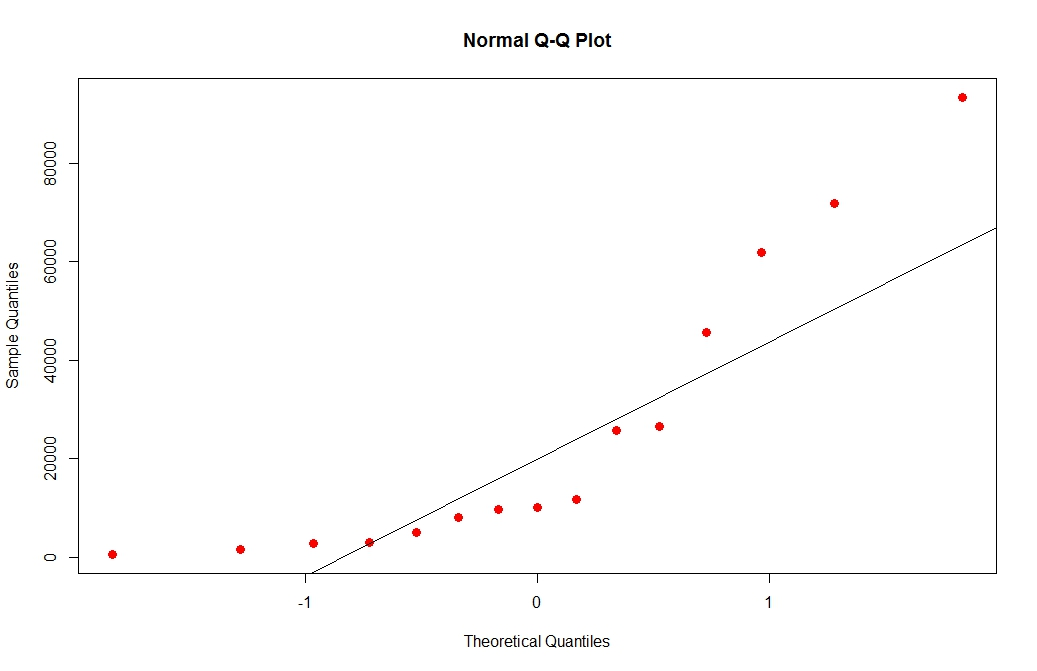
\includegraphics[scale=0.45]{images/MT2016-QQPLOT}
\end{center}

\begin{itemize}
	\item[(iv.)] (1 Mark) Provide a brief description on how to interpret this plot.
	\item[(v.)] (1 Mark) What is your conclusion for this procedure? Justify your answer.
\end{itemize}


\subsection*{Part D (5 Marks)}

% \subsection*{Q9.Robust Regression}
%Write a brief explanation of how robust regression differs from linear models computed using the \emph{Ordinary Least Squares method}, making reference to one particular weighting method only. Provide a description on how this weighting method works.


In certain circumstances, Robust Regression may be used in preference to Ordinary Least Squares Regression. Answer the following questions relating to Robust Regression. 

\begin{itemize}
	%	\item[(i.)] (1 Mark) Describe what these circumstances might be.
	%	\item[(ii.)] (1 Mark) State one difference between OLS and Robust regression techniques, in terms of computing regression equations.
	\item[(i.)] (2 Marks) Explain the process of Huber Weighting for Residuals, stating the algorithm used to compute weightings.
	\item[(ii.)] (3 Marks) Suppose that Huber Weighting, with a tuning constanct of $k=13.45$, was applied to the observations 
	tabulated below. What would be the outcome of the procedure for each case. 
\end{itemize}
\begin{center}
	\begin{tabular}{|c|c|}
		\hline
		Observation ($i$)& Residual ($e_i$)\\ \hline
		
		\phantom{space}	18 	\phantom{space}	 & 	\phantom{space}	-8.011 	\phantom{space}	\\ \hline 
		23 & 16.54 \\ \hline
		25 & -15.11 \\ \hline
		32 & 18.91 \\ \hline
	\end{tabular} 
\end{center}	

	\subsection*{Part E (5 Marks)}
	
	%\subsubsection*{Part A : Outliers}
	\begin{itemize}
		\item[(i.)] (3 Marks) Provide a brief description for three tests from the family of Grubb's  Outliers Tests. Include in your description a statement of the null and alternative hypothesis for each test
		\item[(ii.)] (2 Marks) Describe any required assumptions for tests, and the limitations of these tests.
	\end{itemize}
	
	
	
	% Review of Univariate Normal Distribution
	% Test for Univariate normality
	% - Graphical Procedures
	% - Formal Tests
	% (Later Multivariate Normality)
	% Boxplots, Outliers and Transformations
	%
	% (Hint: there are no outliers in these data sets)
	
\bigskip


	\subsection*{Part F (5 Marks)}
	Numeric Transformations, such as logarithmic transformation, are often used in statistical analysis as an approach for dealing with non-normal data.
	\begin{itemize}
		\item[(i)] (1 Marks) Discuss the importance of numeric transformations, such as logarithmic transformation, in Statistics.
		%	\item[(ii)] Describe the process of transformations
		%	\item[(i.)] (1 Mark) Describe the purpose of Tukey's Ladder (referencing direction and relative strength).
		\item[(ii.)] (3 Marks) Give two examples of a transformation for various types of skewed data (i.e. an example for both types of skewness).
		\item[(iii.)] (1 Mark) Discuss the limitations of numeric transformations.
	\end{itemize}
	


\newpage

\subsection*{Part G (5 Marks)}

\begin{framed}
	\begin{verbatim}
	Int=c(2.1,5.0,9.0,12.6,17.3,21.0,24.7)
	Conc=c(0,2,4,6,8,10,12)
	cor.test(Int,Conc)

Pearson's product-moment correlation

data:  Int and Conc
t = 47.197, df = 5, p-value = 8.066e-08

alternative hypothesis: ................................

95 percent confidence interval:
0.9920730 0.9998421

sample estimates:
cor 
0.9988796 

	\end{verbatim}
\end{framed}

\begin{enumerate}[(i)]
	\item (2 Marks) Describe the Statistical Procedure that you are carrying out. State the Null and Alternative Hypothesis
	\item (1 Mark) By reference to the p-value, interpret the output of this analysis.
	\item (2 Marks) By reference to the 95\% confidence interval
	, interpret the output of this analysis. Explain how you came to this conlcusion
\end{enumerate}
\newpage
(END OF EXAM)
\end{document}	
%======================================================



\section*{Polynomial Regression}
\begin{itemize}
	\item Polynomial regression models are useful in situations where the analyst knows that \textit{\textbf{curvilinear effects}} are present in the response variable.
	\item Polynomial models are also useful as approximating functions to unknown and possible very complex nonlinear relationship.
\end{itemize}


In the context of Statistical Modelling, what is means the ``Law of Parsimony".

What is the Akaike information criterion? How would you use it in statical modelling? How does it differ from other metrics such as the 
coefficient of determination. How would you interpret an AIC value.

compare and contrast forward selection and backward selection as variable selection procedures.

In the context of Statistical Modelling,What is meant by Stepwise regression?

Explain why an adjusted R2 value is often preferred to R2
when comparing
models. 

%- http://www.hkss.org.hk/images/exam/papers/Past/2009/2009_GD_M4_HKSS.pdf



%=============================================================%
Usual assumptions are that the residual (error) terms should be independent,
identically distributed, have zero mean and constant variance, and, if the usual
inferences and tests are to be made, be Normally distributed. 


%-------------------------------------------------------------%
\newpage











\subsection*{Q4. Dixon Q Test For Outliers (4 Marks)}

The typing speeds for one group of 12 Engineering students were recorded both at the beginning of year 1 of their studies. The results (in words per minute) are given below:

\begin{center}
	\begin{tabular}{|c|c|c|c|c|c|c|}
		\hline
		% Subject& A& B& C& D& E &F &G &H \\ \hline
		121 & 146 & 150 &149 &142 &170& 153\\ \hline
		137 & 161 & 156& 165& 137& 178& 159
		\\ \hline
	\end{tabular}
\end{center}
Use the Dixon Q-test to determine if the lowest value (121) is an outlier. You may assume a significance level of 5\%.
%Calculate a 95\% confidence interval for the difference between the mean number of marks obtained by males and females in the population of school leavers as a whole.
%(7 marks)

\begin{itemize}
	\item[i.] (1 Mark) Formally state the null hypothesis and the alternative hypothesis.
	\item[ii.] (1 Mark) Compute the Test Statistic.
	\item[iii.] (2 Mark) By comparing the Test Statistic to the appropriate Critical Value, state your conclusion for this test.
\end{itemize}


	\subsubsection*{Question 1 Part B (5 Marks)}
	
	The typing speeds for one group of 12 Engineering students were recorded both at the beginning of year 1 of their studies. The results (in words per minute) are given below:
	
	\begin{center}
		\begin{tabular}{|c|c|c|c|c|c|}
			\hline
			% Subject& A& B& C& D& E &F &G &H \\ \hline
			149  & 146 & 112 & 142 & 168& 153\\ \hline
			137 & 161 & 156& 165&  170&  159
			\\ \hline
		\end{tabular}
	\end{center}
	Use the Dixon Q-test to determine if the lowest value (118) is an outlier. You may assume a significance level of 5\%.
	\begin{itemize}
		\item[(i.)](1 Mark)	State the Null and Alternative Hypothesis for this test.
		\item[(ii.)](2 Marks) Compute the test statistic
		\item[(iii.)](1 Mark) State the appropriate critical value.
		\item[(iv.)](1 Mark) What is your conclusion to this procedure.
	\end{itemize}
	\newpage

\bigskip
\subsection*{Q1. Dixon Q Test For Outliers (4 Marks)}

The typing speeds for one group of 12 Engineering students were recorded both at the beginning of year 1 of their studies. The results (in words per minute) are given below:

\begin{center}
	\begin{tabular}{|c|c|c|c|c|c|}
		\hline
		% Subject& A& B& C& D& E &F &G &H \\ \hline
		118 & 146 & 149 & 142 & 170& 153\\ \hline
		137 & 161 & 156& 165&  178& 159
		\\ \hline
	\end{tabular}
\end{center}
Use the Dixon Q-test to determine if the lowest value (118) is an outlier. You may assume a significance level of 5\%.
\begin{itemize}
	\item[i.](1 Mark)	State the Null and Alternative Hypothesis for this test.
	\item[ii.](1 Marks) Compute the test statistic
	\item[iii.](1 Mark) State the appropriate critical value.
	\item[iv.](1 Mark) What is your conclusion to this procedure
\end{itemize}

%Calculate a 95\% confidence interval for the difference between the mean number of marks obtained by males and females in the population of school leavers as a whole.
%(7 marks)

\newpage
%\newpage


\section*{Formulae and Tables}
\subsection*{Critical Values for Dixon Q Test}
{
	\Large
	\begin{center}
		\begin{tabular}{|c|c|c|c|}
			\hline  N  & $\alpha=0.10$  & $\alpha=0.05$  & $\alpha=0.01$  \\ \hline
			3  & 0.941 & 0.970 & 0.994 \\ \hline
			4  & 0.765 & 0.829 & 0.926 \\ \hline
			5  & 0.642 & 0.710  & 0.821 \\ \hline
			6  & 0.560 & 0.625 & 0.740 \\ \hline
			7  & 0.507 & 0.568 & 0.680  \\ \hline
			8  & 0.468 & 0.526 & 0.634 \\ \hline
			9  & 0.437 & 0.493 & 0.598 \\ \hline
			10 & 0.412 & 0.466 & 0.568 \\ \hline
			11 & 0.392 & 0.444 & 0.542 \\ \hline
			12 & 0.376 & 0.426 & 0.522 \\ \hline
			13 & 0.361 & 0.410 & 0.503 \\ \hline
			14 & 0.349 & 0.396 & 0.488 \\ \hline
			15 & 0.338 & 0.384 & 0.475 \\ \hline
			16 & 0.329 & 0.374 & 0.463 \\ \hline
		\end{tabular} 
	\end{center}
}
\newpage
\subsection*{Critical Values for Chi Square Test}
{



\end{document}
\subsection*{Confidence Intervals}
{\bf One sample}
\begin{eqnarray*} S.E.(\bar{X})&=&\frac{\sigma}{\sqrt{n}}.\\\\
S.E.(\hat{P})&=&\sqrt{\frac{\hat{p}\times(100-\hat{p})}{n}}.\\
\end{eqnarray*}
{\bf Two samples}
\begin{eqnarray*}
S.E.(\bar{X}_1-\bar{X}_2)&=&\sqrt{\frac{\sigma^2_1}{n_1}+\frac{\sigma_2^2}{n_2}}.\\\\
S.E.(\hat{P_1}-\hat{P_2})&=&\sqrt{\frac{\hat{p}_1\times(100-\hat{p}_1)}{n_1}+\frac{\hat{p}_2\times(100-\hat{p}_2)}{n_2}}.\\\\
\end{eqnarray*}
\subsection*{Hypothesis tests}
{\bf One sample}
\begin{eqnarray*}
S.E.(\bar{X})&=&\frac{\sigma}{\sqrt{n}}.\\\\
S.E.(\pi)&=&\sqrt{\frac{\pi\times(100-\pi)}{n}}
\end{eqnarray*}
{\bf Two large independent samples}
\begin{eqnarray*}
S.E.(\bar{X}_1-\bar{X}_2)&=&\sqrt{\frac{\sigma^2_1}{n_1}+\frac{\sigma_2^2}{n_2}}.\\\\
S.E.(\hat{P_1}-\hat{P_2})&=&\sqrt{\left(\bar{p}\times(100-\bar{p})\right)\left(\frac{1}{n_1}+\frac{1}{n_2}\right)}.\\
\end{eqnarray*}
{\bf Two small independent samples}
\begin{eqnarray*}
S.E.(\bar{X}_1-\bar{X}_2)&=&\sqrt{s_p^2\left(\frac{1}{n_1}+\frac{1}{n_2}\right)}.\\\\
s_p^2&=&\frac{s_1^2(n_1-1)+s_2^2(n_2-1)}{n_1+n_2-2}.\\
\end{eqnarray*}
{\bf Paired sample}
\begin{eqnarray*}
S.E.(\bar{d})&=&\frac{s_d}{\sqrt{n}}.\\\\
\end{eqnarray*}
{\bf Standard Deviation of case-wise differences (computational formula)}
\begin{eqnarray*}
s_d = \sqrt{ {\sum d_i^2 - n\bar{d}^2 \over n-1}}.\\\\
\end{eqnarray*}
\end{document}
% -- Part 3 - Confidence Interval

% 2 Marks Using previously calculated values, compute the confidence interval
